The origin of cartography lays far back in the history of visualization as shown in chapter \ref{s:history} on page \pageref{s:history}. Today's understanding of modern cartography began in the late 18\textsuperscript{th} century with the attempt to show more than one attribute in a map. \citeauthor{Longley2005} say, that topography has long been understood as an important aspect of war strategy. Battles and wars could be decided on the information of the topology. A commander had to position his units wisely in order to exploit all geographical circumstances and thus have an advantage over his opponent \iacite{Longley2005}.
in the middle of the 20\textsuperscript{th} century, the Soviets, Fascist Italy and Nazi Germany all used map to foster national pride. This could furthermore be used to justify their expansionism \iacite{Crampton2015}.
Today, national organisations produce a variety of maps for different reasons with a very high focus of map accuracy (see chapter \ref{s:map-accuracy} on page \pageref{s:map-accuracy} for more information) and transmittal of relvant information.

The field of cartography can be divided into two major subcategories:
\begin{enumerate}
\ditem{General cartography} is associated with maps that are constructed for commonalty. These type of maps often contain a variety of features and display many reference and location systems. An abstract definition of general maps is that those kind of maps show the variety of phenomena of either geological, geographical or policital nature together \iacite{Thrower2008}.

\ditem{Thematic cartography} focuses on a specific subject area, often called theme. Thus it involves maps which emphasize spatial variation of geographic distributions. \citeauthor{BartzPetchenik1979} describes thematic maps compared to general (or reference) maps as "in place, about space". She says, that the a general map is characterized by the fact that it shows you where something is in space, according to the example. However, thematic maps will tell a story about that specific place \iacite{BartzPetchenik1979}.
In order to make a connection to the abstract definition \citeauthor{Thrower2008} made for general maps, thematic maps could be described as follows:
Those kind of maps (thematic) use the base data only as points of references. Base data could be coastlines, boundaries and places. Phenomena of all kind are being mapped onto the reference \iacite{Thrower2008}.
\end{enumerate}

The following sections in this chapter should provide general knowledge about different types of maps, scaling, projecting, generalization and symbolization and accuracy. This knowledge is needed in order to understand the implementation of the partical part of this thesis.

\subsubsection{Methods of thematic maps}
The two major categories of cartography are general cartography and thematic cartography, which are introduced in chapter \ref{s:cartography} on page \pageref{s:cartography}. This categorization can be directly mapped from cartography to maps. The main objective of this chapter is to give an overview of different thematic maps and their usage. These maps can be subdivided into univariate and multivariate maps.

\subsubsubsection{Univariate Thematic Map Types}
Univariate maps are only dependent on one variable, except for the map variables like latitude and longitude and suchlike.

\sectionparagraph{Dot density map}
The first dot map in history is shown in figure \ref{fig:cholera-map} on page \pageref{fig:cholera-map}. It was the first map of its kind and could help in the display of disease outbreaks. This type of univariate thematic map uses points or dots to map discrete data. Attribute values of the given data determine the number of dots displayed in a specific regions. All dots need to be the same size. To explain the two different types of dot maps, imagine a dataset of customers where each customer has a location:

\begin{enumerate}
\ditem{One-to-one} \hfill \\
Each dot on the map represents exactly one item of the represented theme. Considering the example dataset mentioned above, every customer would be represented by exactly one dot.
\ditem{One-to-many} \hfill \\
Each dot on the map represents an aggregate of information. Therefore this type of dot map could be used with the aggregation of customers in a specific location. Thus the map maker needs to make the decision how many customers are aggregated, or rather how many customers are represented by one dot.
\end{enumerate}

Both types of dot density maps share the purpose, that they are not a tool to determine exact quantities. Getting the exact amount of dots in a high density area is a very cumbersome task and users often tend to underestimate dot totals as density increases \iacite{McMaster2001}. However, it is a very common technique for viewing the clustering, dispersion, linearity, and general pattern of a distribution. The technique appeared first in the 19\textsuperscript{th} century and is today accepted as one of the primary techniques for representing geographic patterns \iacite{Tyner2010}.

The map maker can use dots in a dot density map with a different type of level of detail. This means, that dots do not necessarily need to have an exact location. If he or she wants to discover a pattern on a state-wide level of detail, dots can be placed anywhere in their corresponding states, as long as they do not leave their state boundaries.
Another location based decision the map maker needs to make is, if the dots should use some kind of pseudo-random placement in case of overlapping. This decision is based on a maximum overlap constraint. It can be thought of as a random placement of dots in a square without violating the constraint.

According to \citeauthor{Tyner2010}, ther are some main design principles for dot maps that should be considered:
\begin{itemize}
\item The size of the dot.
\item The value assigned to the dot. This also includes the correct use of the two different types of dot maps.
\item The location of the dot on the map in case of an aggregated level of detail of the map.
\item The aggregated units in case of a one-to-many dot map. This design principle can be thought of as using a legend in order to tell the aggregated value one dot represents.
\end{itemize}
Changing any one of these can change the overall appearance and interpretation of the map \iacite{Tyner2010}.

The main advantage of this type of map is the understandability. It requires little to no cognitive effort by the user to read the map when compared to other types. Specific advantages of dot maps are the good measure of density and the loose coupling between the size of a dot and its represented value.
However, reading specific information from those maps is not an easy task as mentioned before. Additionally, if a map uses some kind of random placement without any hint in the visualization, map readers may potentially infer the locations of dots as precise locations of the mapped phenomenon. To counteract the second drawback, dot density maps with random placement of dots should consider the acual occurence of the mapped phenomenon, e.g. dots should not be placed in lakes for a map of population.

\sectionparagraph{Graduated symbol or proportional symbol map}
Figure \ref{fig:first-mixture} on page \pageref{fig:first-mixture} shows a special kind of a proportional symbol map. According to figure \ref{fig:va-channels} on page \pageref{fig:va-channels}, this type of map uses the visual channel of size to represent differences of discrete data. Again, this type of map can be subdivided into two categories: classed and unclassed. Classed ones are known as range-graded or graduated symbol maps, whereas unclassed ones are called proportional symbol maps. The latter one uses a symbol size proportional to the value of the attribute being mapped \iacite{Dutton.2014}.
Although circles are the most typical symbol used, it is possible to use any type of symbol, ranging from abstract, geometric symbols to pictographic symbols. Figure \ref{fig:different-symbols} on page \pageref{fig:different-symbols} shows two proportional symbol maps showing the same phenomenon. The left part of this figure uses the common circle as symbol, while the right side uses a pictogram. Albeit the established circle because of their compactness due to their low perimeter to area ratio, \citeauthor{Dutton.2014} says, that squares or bars are easier to estimate the size of the symbol.


\begin{figure}[!htb]
\centering
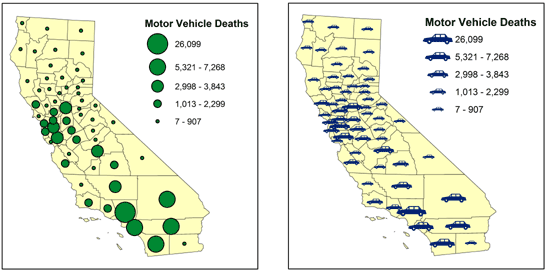
\includegraphics[height=5cm,keepaspectratio]{images/psm/symbols.png}
\caption[
    Two types of proportional symbol maps with different symbols \iacite{Dutton.2014}.
]{Two types of proportional symbol maps with different symbols.}
\label{fig:different-symbols}
\end{figure}

Another consideration in terms of symbol used is the fact, that squares and bars tend to run off the page with large values earlier than circles might \iacite{Dutton.2014}. \citeauthor{FLANNERY1971} introduced a scaling factor for proportional circles for better estimation of the value. However, this correction may not be very effective, because the correction itself does not consider the map context. A phenomenon related to the importance of context is known as the ebbinghaus illusion. Figure \ref{fig:ebbinghaus} on \pageref{fig:ebbinghaus} shows such an illusion. Both central circles actually have the same size, but because of the context of each side, the central circles appear different.

\begin{figure}[!htb]
\centering
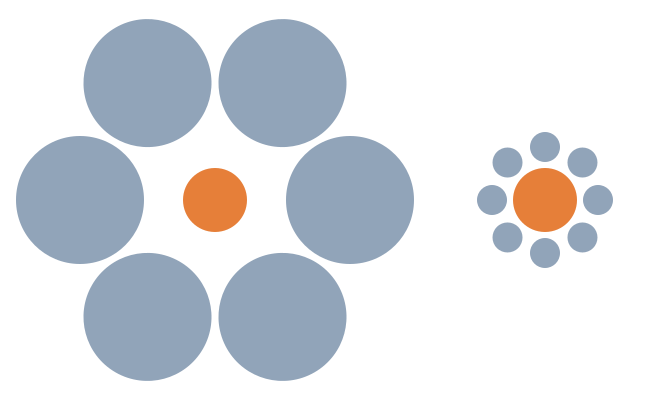
\includegraphics[height=5cm,keepaspectratio]{images/psm/ebbinghaus.png}
\caption[
    Ebbinghaus illusion, Urldate: 07.2016 \newline
    \small\texttt{\url{https://upload.wikimedia.org/wikipedia/commons/b/bc/Mond-vergleich.svg}}
]{Ebbinghaus illusion}
\label{fig:ebbinghaus}
\end{figure}

In order to combat the problem of value estimation, there are two major choices:
\begin{enumerate}
\item A legend could show proportional symbols which represent the different values of the mapped phenomenon. One possibility would be to display the smallest symbol, the largest symbol and some symbols at intermediate values.
\item Another alternative is to use range-graded symbols. Therefore the data needs to be classified, but in exchange the estimation problem is completly avoided. This alternative still needs consideration in the size of symbols, because each symbol should still be differentiable from each other.
\end{enumerate}

Based on the given knowledge about proportional and gradient symbol maps, it is possible to derive some main design principles:
\begin{itemize}
\item The estimation of the value of a symbol is key for this type of map. This is most easily accomplished with geometric symbols.
\item Use a legend with exmaples to increase the reader's ability to correctly estimate the value of a symbol.
\end{itemize}

A close related problem to the user's estimation problem is the actual scaling technique used. According to \citeauthor{Dent2008} the three most commong techniques used are
\begin{enumerate*}
\item absolute scaling,
\item apparent magnitude scaling and
\item range grading \iacite{Dent2008}.
\end{enumerate*}

\begin{enumerate}
\ditem{Absolute scaling} makes each symbol fit it's dat value on the scale being used. This means, that a symbol representing four items in a dataset is twice as big as a symbol representing two.
\ditem{Apparent magnitude scaling} compensates for human error interpretation in scale. Using this technique, a symbol having twice as much in value is not twice as big, because it would appear smaller, leading to interpretation error. This type of scaling takes this error into account and increased the size of a symbol by more than the proportional amount \iacite{Krygier.2007}.
\ditem{Range grading} classifies the data into a fixed amount of groups. Each group has a fixed range of values and the same symbol to represent. The groups only differ in the range of values they represent and the size of the symbols.
\end{enumerate}

The main advantage of a proportional symbol map is the flexibility it comes along with. Possible data can either be numerical or categorical nature. Even the way the data is used is adjustable. An item can be mapped on a precise location or to geographic areas, depending on the level of detail.
Comparing proportional symbol maps with dot density maps, one advantage is observable: the estimation problem of dot density maps is less tedious. However, if proportional symbol maps are put in comparison with choropleth maps, they also have an advantage: the size of the enumeration unit does not matter. This problem will be explained in detail in chapter \ref{s:choropleth} on page \pageref{s:choropleth}.

\sectionparagraph{Choropleth map}
Choropleth maps are extremely popular, probably the most common thematic map in use today. That's good because it means your audience is likely to understand them. One reason they're popular is that much of our geodata is reported by enumeration units, such as census data, and so we are accustomed to thinking of the world as divided into spatial units like census tracts, counties, and provinces. However, most cartographers would argue choropleth maps are over-used and commonly misused if the geographic phenomena being mapped aren't intrinsically tied to enumeration units: For example, communicable diseases, soil types, or age demographics don't care much about county lines or zip codes and rarely do they change abruptly at those human-created boundaries. By comparison, tax rates are very closely tied to enumeration units, do change abruptly, and make perfect sense as a choropleth map. The less the thing you are mapping is tied to enumeration units, the less sense a choropleth map makes.

These are maps, where areas are shaded according to a prearranged key, each shading or colour type representing a range of values. Population density information, expressed as 'per km²,' is appropriately represented using a choropleth map. Choropleth maps are also appropriate for indicating differences in land use, like the amount of recreational land or type of forest cover.



For continuous data, two mapping techniques are commonly used: choropleth and isarithmic mapping. This chapter will only cover choropleth mapping because the practical part of this thesis will not feature isarithmic mapping.


The choropleth method involves applying value or color
intensity to enumeration units (census tracts, counties, states, nations) based on some statistical
value. The higher an enumeration unit’s data value, the darker or more saturated the color value.
Fundamental to every choropleth method are the concepts of data standardization and
classification.
All choropleth data must be standardized. We repeat: a choropleth map may never – ever –
be used to map count data. If one maps raw data using the choropleth method, the visualization
will suffer from an inherent areal bias. Not all enumeration units are the same size; thus, some
enumeration units will naturally have more count data than others simply due to their areal
extent. For instance, Texas and California have greater populations than Rhode Island or
Connecticut. This should not be a surprise – Texas and California have huge areas compared to
the other two states. If you standardize the data by area, however, Connecticut and Rhode Island
are far more populated when it comes to the number of people per square kilometer. If you are
interested in comparing the raw number of people living in states, you should use proportional
symbols.
\label{s:choropleth}

\subsubsubsection{Multivariate Thematic Map Types}

\subsubsection{Map Scale}
\label{s:map-scale}
Maps are scale models of the earth by itself. Scaling is a simple concept per se but is complicated by the earth's curvature. It will control multiple things e.g. how much data can be mapped in a map frame, the size of symbols, the overlap of symbols, and so forth \iacite{Longley2005}. Without considering curvature, scaling can be explained as the reduction or enlargement of real world objects by a constant amount.

The following list shows two different representations of scales:
\begin{enumerate}
\ditem{Bar scale} \hfill \\
Figure \ref{fig:bar-scale} on page \pageref{fig:bar-scale} visually shows the scale of a map. The first black bar indicates, that $1$cm in the map represents $100$cm in real world. It includes everything needed: the ratio, the unit of measure and a visual example of both.

\begin{figure}[!htb]
\centering
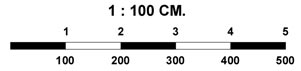
\includegraphics[width=0.4\textwidth,keepaspectratio]{images/methods/scalebar.jpg}
\caption[
    Bar scale.
]{Bar scale.}
\label{fig:bar-scale}
\end{figure}

\ditem{Lexical scale} \hfill \\
Words describing a ratio are known as lexical scales. $1:1000$ can be interpreted as as scale, where $1$ unit of measure on the map, represents $1000$ units of measure in real world. The unit of measure is very important to mention in a lexical scale.
\end{enumerate}

However, taking the earth's curvature into consideration, scaling large areas result in noticeable distortions. The distribution of distortion is dependent on the map projection (see chapter \ref{s:map-projections} on page \pageref{s:map-projections} for more information).

Choosing the correct type of scale depends on several factors: the theme and purpose of the map, data resolution, and the specified format. If a map is designed for navigation, it will need more detail than if it is designed to show an overview of a national park \iacite{Tyner2010}.

\subsubsection{Map Projections}
As chapter \ref{s:map-scale} on page \ref{s:map-scale} already mentioned, the map scale is heavily dependent on the map projection. The true figure of the earth is not a regular shape like a sphere or an ellipsoid. It has a seperate shape, which is called geoid.
From a general point of view, every projection distorts the earth somehow, but the advantage of projection is, that any point can be exactly recreated at any given time, due to the fact, that the projection affects the whole earth.
A projection consists of four main properties:
\begin{enumerate*}
\item area,
\item form,
\item distance and
\item directions.
\end{enumerate*}
Every projection affects all its properties in some way. Some of them preserve area and form while distorting distances and directions \iacite{Snyder1987}.

In order to understand the sub-chapters explaining different types of projections, some terms need to be explained first:

\begin{enumerate}

\ditem{Conformal} \hfill \\
If a projection is conformal, it preserves local angles in the map. This can be thought of preserving the general shape of e.g. an island. Some parts of an island may get larger or smaller due to a conformal projection, but the recognizability of the island is still given \iacite{Snyder1987}.

\ditem{Loxodromes} \hfill \\
According to the Merriam Webster Online Dictionary\footnote{See \href{http://www.merriam-webster.com/}{Merriam Webster Dictionary}} a loxodrome is also called rhumb line and can be defined as "[\ldots] a line on the surface of the earth that follows a single compass bearing and makes equal oblique angles with all meridians". A more practical example of loxodromes is to imagine a sailing route between two points. This line is shown as a straight line, as long as the intended course of the ship remains constant with respect to north.

\ditem{Equal-Area} \hfill \\
If a map bares the name equal-area, it means that it preserves area by distorting shapes.

\end{enumerate}

For most thematic maps irregularities of the earth's shape are ignored, as long as geodetic accuracy is not related to the purpose of the map \iacite{Snyder1987}. Figure \ref{fig:projections-base} on page \ref{fig:projections-base} is in the subsections and helps to explain some major characteristics of the different types of projections. Every projection is only listed with its characteristics. These will not be discussed in detail, as it would go beyond the scope of this thesis.

\begin{figure}[!htb]
\centering
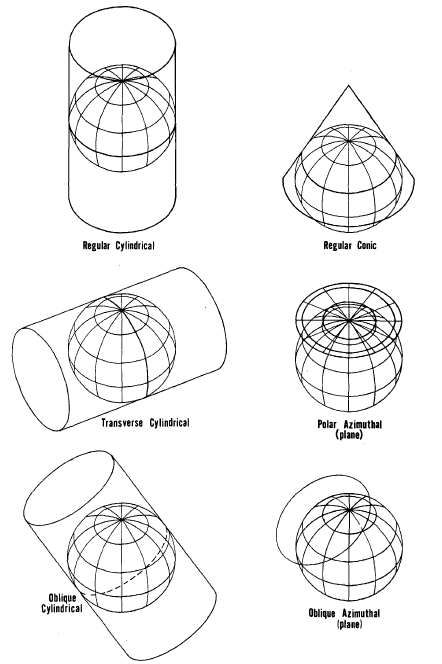
\includegraphics[width=0.8\textwidth,keepaspectratio]{images/methods/mappings.png}
\caption[
    Projection of the earth onto the three major surfaces \iacite{Snyder1987}.
]{Projection of the earth onto the three major surfaces.}
\label{fig:projections-base}
\end{figure}

\subsubsubsection{Cylindrical map projections}
The main concept of cylindrical map projections consist "[\ldots] of meridians which are equidistant parallel straight lines, crossed at right angles by straight parallel lines of latitude, generally not equidistant \iacite{Snyder1987}".
In general, cylindrical map projections can be thought of unrolling a cylinder which has been wrapped around a geoid, touching at the equator (see figure \ref{fig:projections-base} on page \pageref{fig:projections-base}).
The primary use for this type of projection is to either map the complete world, or for maps along narrow strips of a great circlel arc, such as the equator.

The following list will only feature two common projections accordingly to cylindrical projections with a short description taken from \citeauthor{Snyder1987} \iacite{Snyder1987}:

\begin{enumerate}

\ditem{Mercator Projection} \hfill \\
It is a cylindrical, conformal projection where meridians are equally spaced straight lines, whereas parallels are unequally spaced straight lines. The scale of the map is only true along the equator and loxodromes are straight lines. The biggest distortion appears close to the poles. The major advantage according to \citeauthor{Snyder1987} is the navigational feature that loxodromes are straight lines \iacite{Snyder1987}. Figure \ref{fig:projections-mercator} on page \pageref{fig:projections-mercator} shows an example mercator projection of the earth.

\begin{figure}[!htb]
\centering
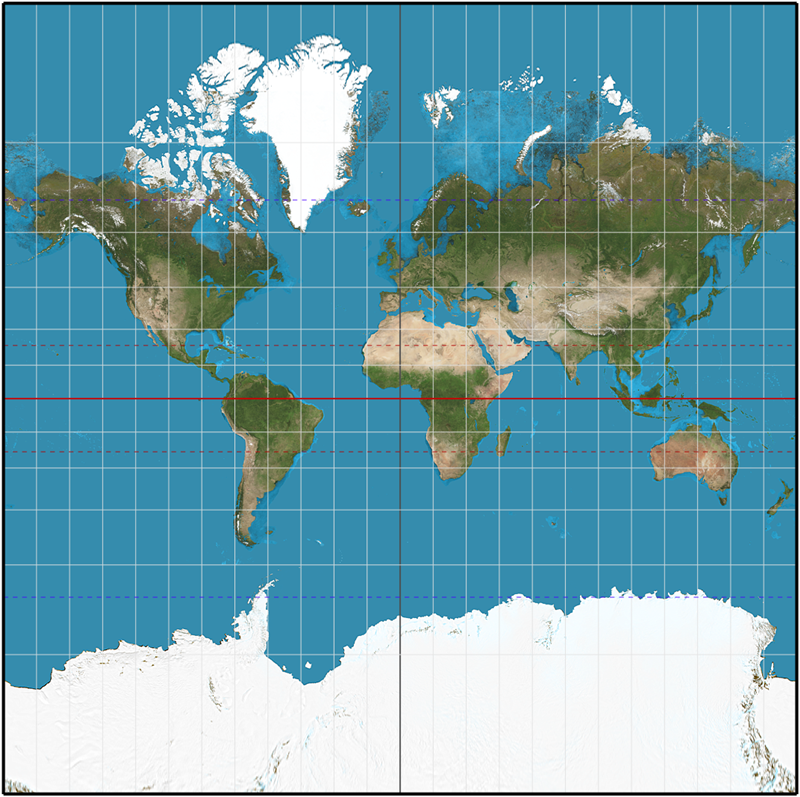
\includegraphics[height=5cm,keepaspectratio]{images/methods/projections/mercator.png}
\caption[
    Mercator projection, Urldate: 07.2016 \newline
    \small\texttt{\url{https://upload.wikimedia.org/wikipedia/commons/f/f0/MercNormSph.png}}.
]{Mercator projection}
\label{fig:projections-mercator}
\end{figure}


\ditem{Transverse Mercator Projection} \hfill \\
This projection is similar to the basic mercator projection except the main difference of a transverse, cylindrical and conformal projection. The central meridian and each meridian 90 degrees east and west of the central meridian are straight lines. All other meridians and parallels are complex curves. The scale of the map is only true along the central meridian \iacite{Snyder1987}. Figure \ref{fig:projections-mercator-transverse} on page \pageref{fig:projections-mercator-transverse} illustrates the described characteristics.

\begin{figure}[!htb]
\centering
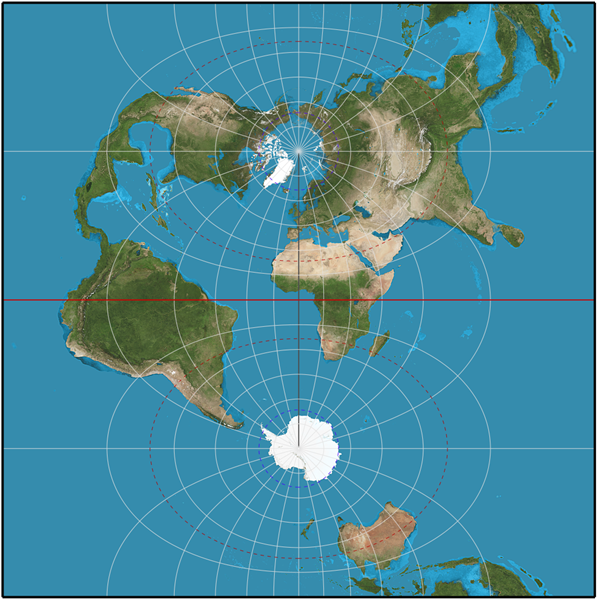
\includegraphics[height=5cm,keepaspectratio]{images/methods/projections/mercator-transverse.png}
\caption[
    Transverse mercator projection, Urldate: 07.2016 \newline
    \small\texttt{\url{https://upload.wikimedia.org/wikipedia/commons/1/15/MercTranSph.png}}.
]{Mercator projection}
\label{fig:projections-mercator-transverse}
\end{figure}


\end{enumerate}

\subsubsubsection{Conic map projections}
Conic projections are preferred over cylindrical ones if the purpose of the map is to show a region for which the greatest areal extent is from east to west in the temperature zone. This projection type makes use of "[\ldots] arcs of concentric circles for parallels of latitude and equally spaced straight radii of these circles for meridians \iacite{Snyder1987}." The main distinctive feature is based on placing a cone on the top of a globe representing the earth (see figure \ref{fig:projections-base} on page \pageref{fig:projections-base}).

The following list will only feature two common projections with a short description taken from \citeauthor{Snyder1987} \iacite{Snyder1987}:

\begin{enumerate}
\ditem{Albers Equal-Area Projection} \hfill \\
This projection, as seen in figure \ref{fig:projections-albers-ea} on page \pageref{fig:projections-albers-ea}, is a conic, area-preserving one where parallels are unequally spaced arcs of concentric circles, whereas meridians are equally spaced radii of the same circles. It features no distortion in scale or shape along two standard parallels, normally, or along just one. Both poles are arcs of circles. The projection is used for regions with predominant east-west expanse \iacite{Snyder1987}.

\begin{figure}[!htb]
\centering
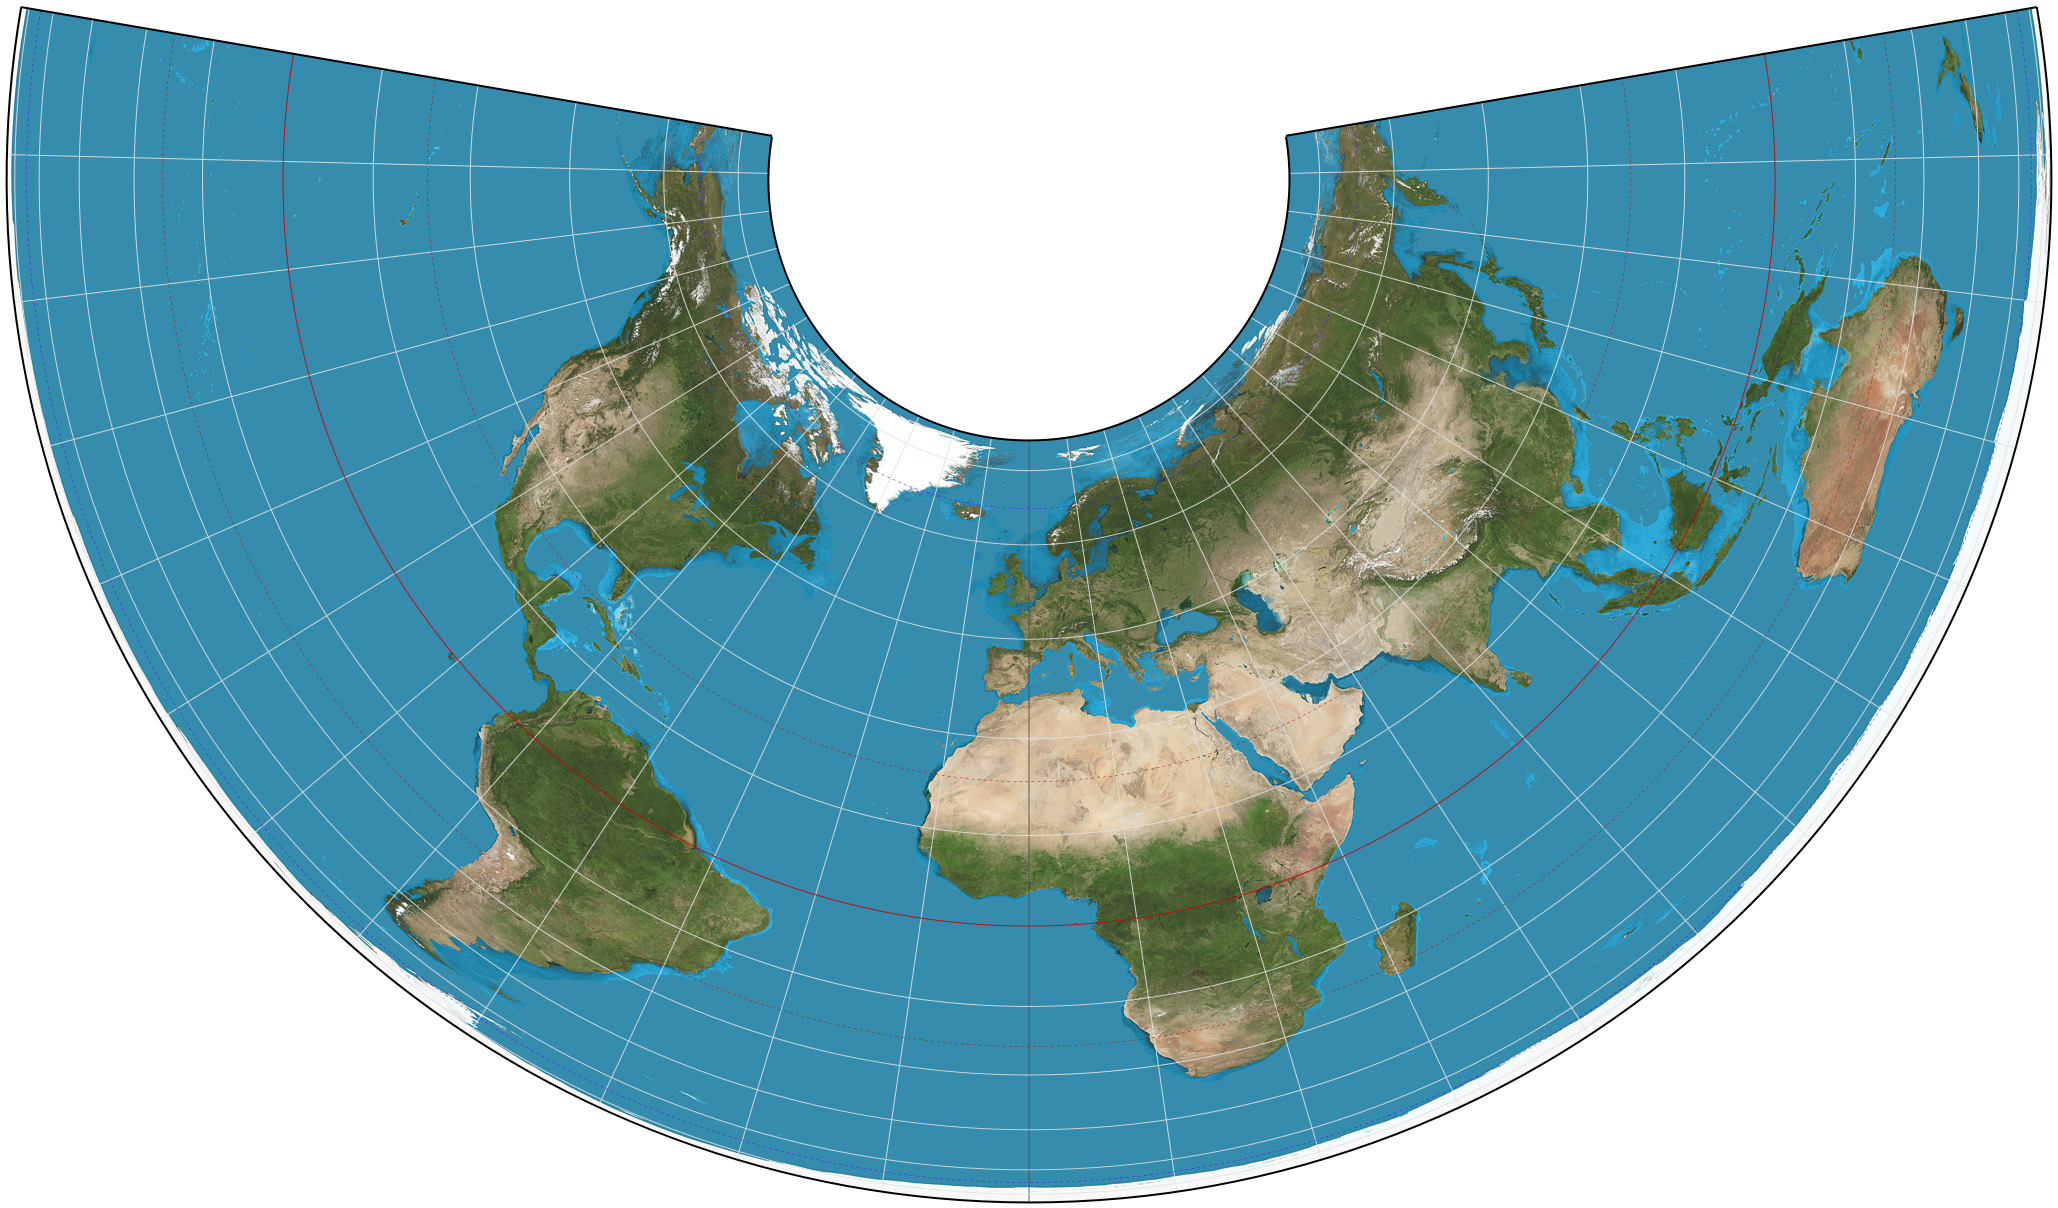
\includegraphics[height=5cm,keepaspectratio]{images/methods/projections/albers.jpg}
\caption[
    Albers equal-area projection, Urldate: 07.2016 \newline
    \small\texttt{\url{https://upload.wikimedia.org/wikipedia/commons/1/1f/Albers_projection_SW.jpg}}.
]{Albers equal-area projection}
\label{fig:projections-albers-ea}
\end{figure}

\ditem{Equidistant Conic Projection} \hfill \\
Equidistant conic projection displays parallels, including poles, as arcs of concentric circles evenly spaced along the meridians. Like the albers equal-area projection, equidistant projection also displays meridians as equally spaced radii of the same circles and thereby cutting parallels at right angles. The scaling of the map is true along all meridians and along one or two standard parallels \iacite{Snyder1987}. Figure \ref{fig:projections-equidistant} on page \pageref{fig:projections-equidistant} shows similarities to the albers equal-area projection. The major distinction is the distortion of direction, area and shape according to the distance from standard parallels.

\begin{figure}[!htb]
\centering
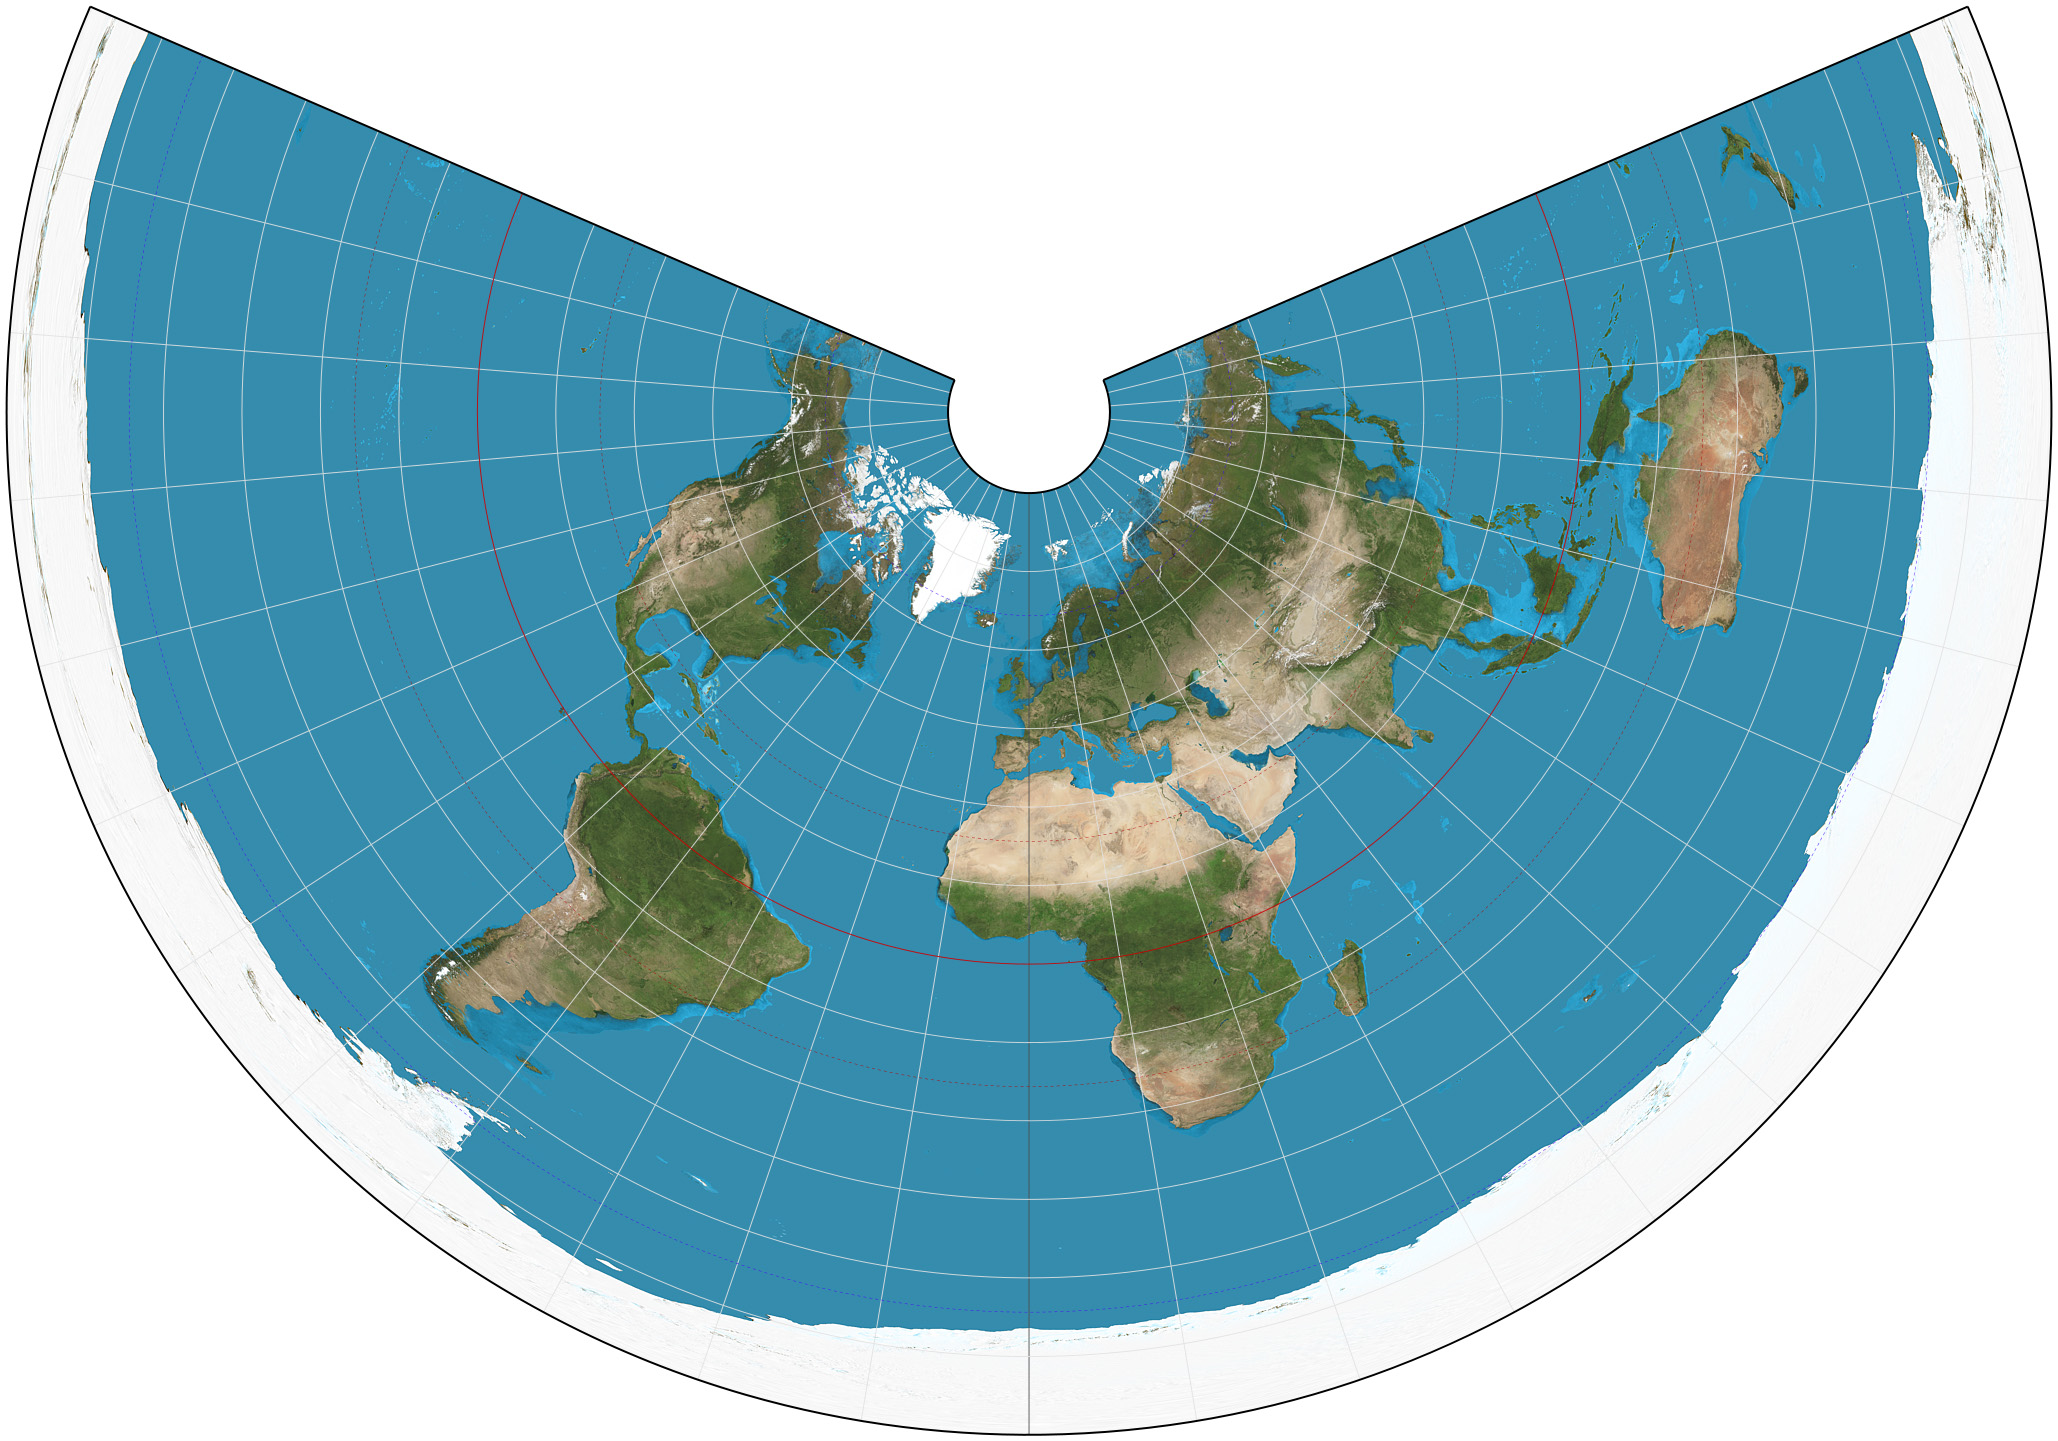
\includegraphics[height=5cm,keepaspectratio]{images/methods/projections/equidistant.jpg}
\caption[
    Equidistant conic projection, Urldate: 07.2016 \newline
    \small\texttt{\url{https://upload.wikimedia.org/wikipedia/commons/d/d8/Equidistant_conic_projection_SW.JPG}}.
]{Equidistant conic projection}
\label{fig:projections-equidistant}
\end{figure}

\end{enumerate}
\subsubsubsection{Azimuthal and related map projections}
Even though cylindrical and conic projections are related to cylinders and cones wrapped around the globe, azimuthal projections are mapped onto a plane. This plane usually is placed tangential at either pole, the equator, or any intermediate point. Each placement bears a different name and are called polar, equatorial and oblique aspects respectively. This type of projection attracted attention with the rise of radio transmission. This is due to the fact, that those type of projections show the direction from the center of the projection to any other point on the map correctly. Figure \ref{fig:projections-azimuthal} on page \pageref{fig:projections-azimuthal} illustrates a polar azimuthal projection. All meridians are straight lines and radiate at their true angles from the center, whereas parallels are concentric circles. Most azimuthal projections do not have standard parallels or standard meridians, because each map has only one standard point. Azimuthals are not suitable for regions with predominant expanse in one direction, because they will maximize distortion \iacite{Snyder1987}.

\begin{figure}[!htb]
\centering
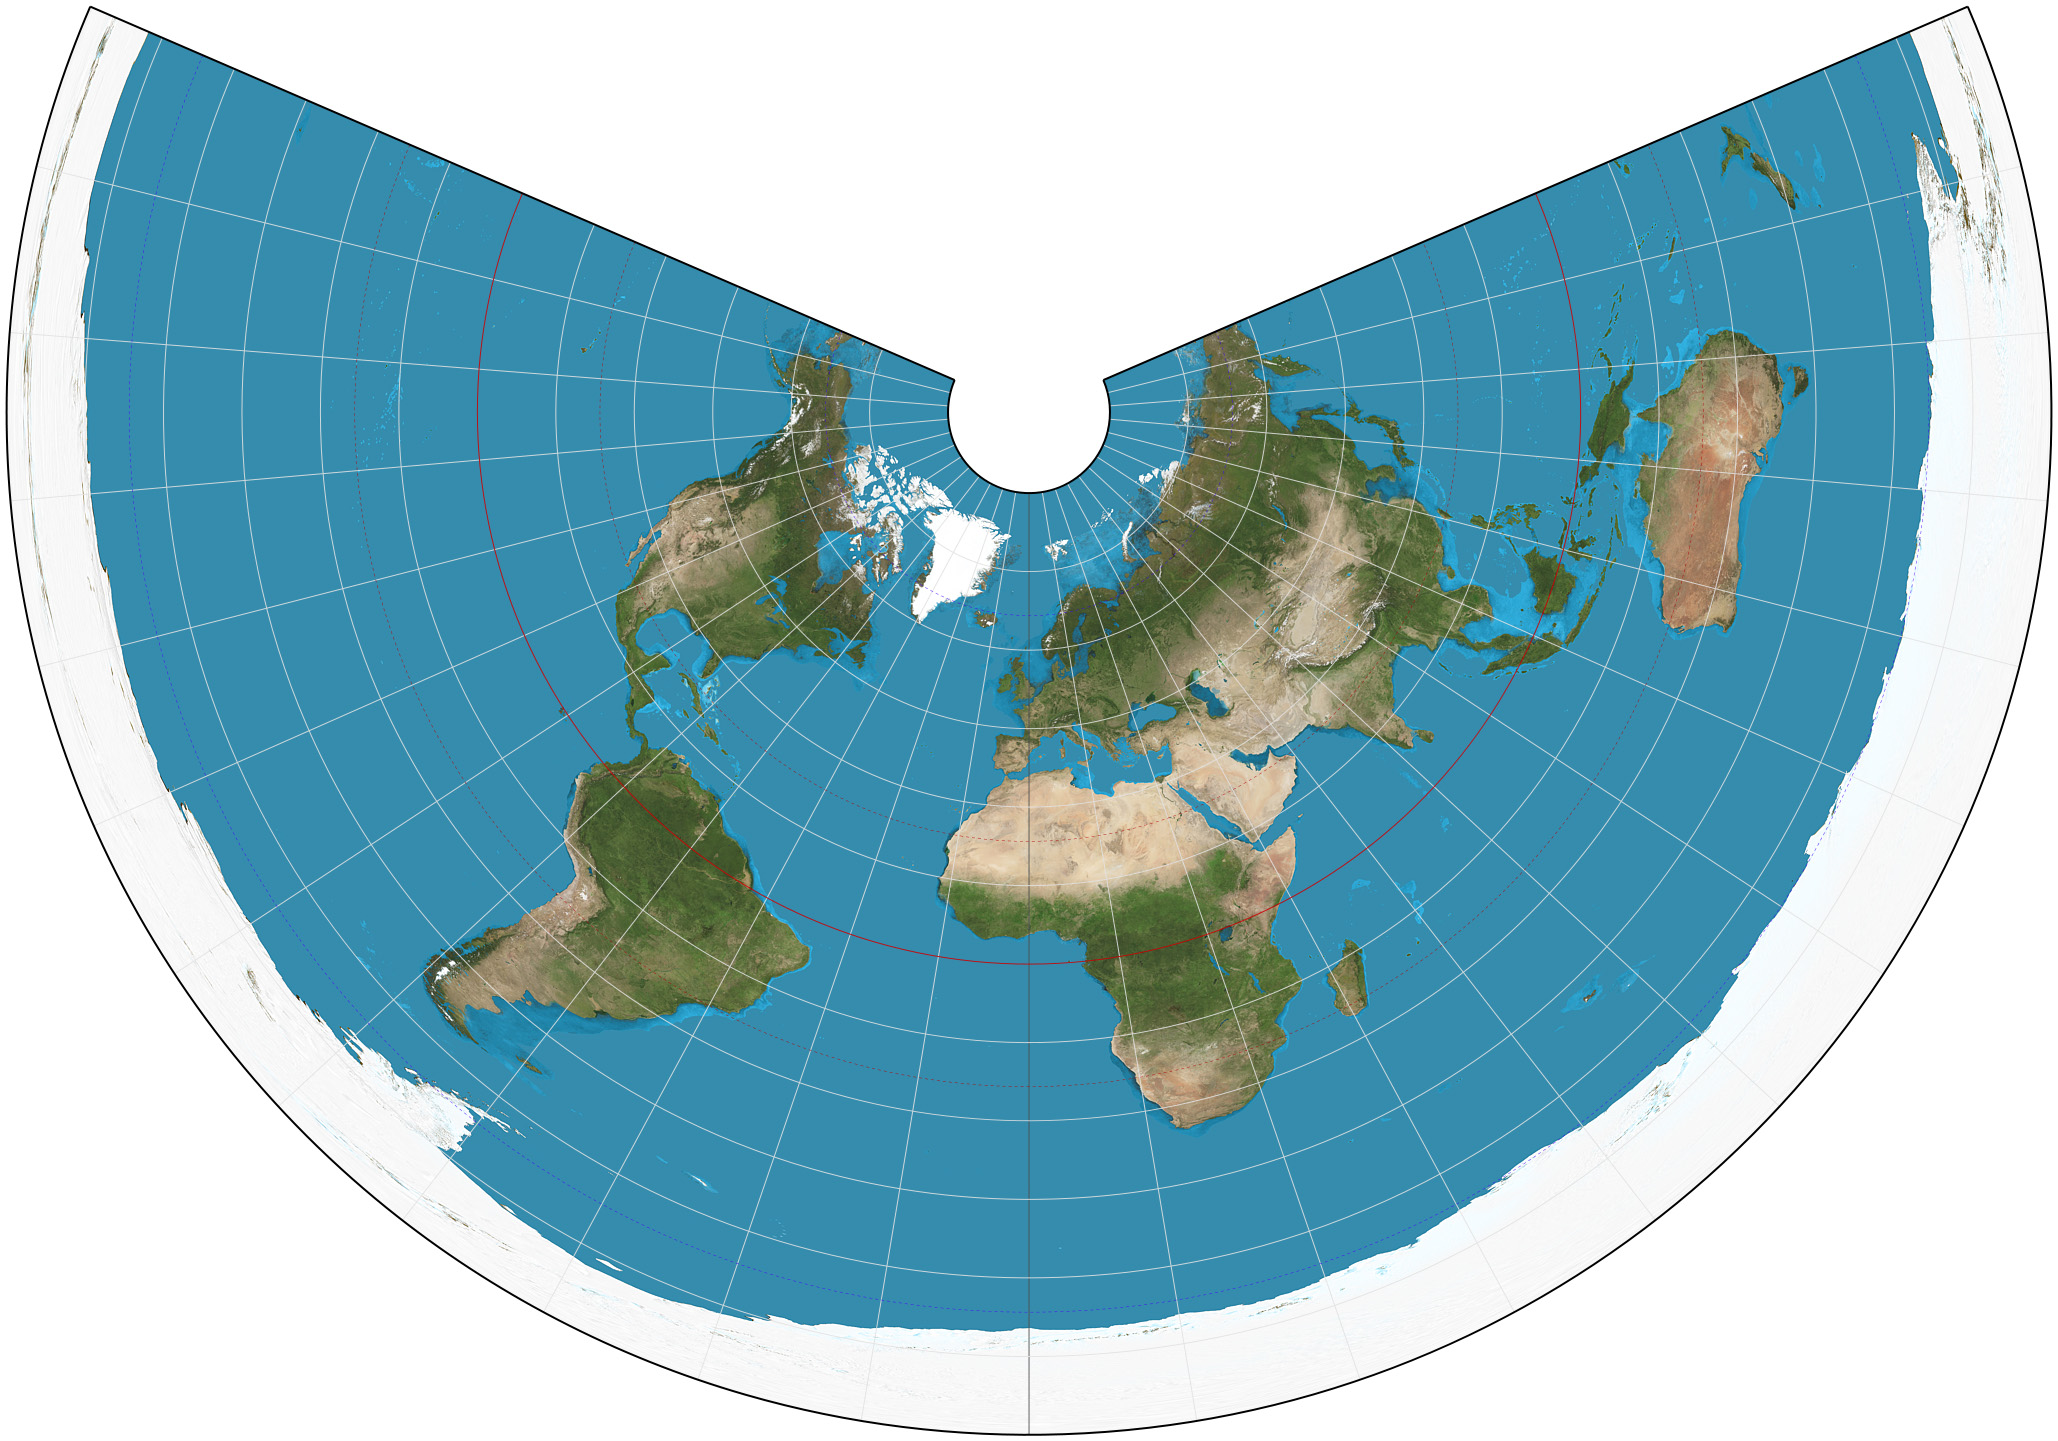
\includegraphics[height=5cm,keepaspectratio]{images/methods/projections/equidistant.jpg}
\caption[
    Azimuthal projection, Urldate: 07.2016 \newline
    \small\texttt{\url{https://upload.wikimedia.org/wikipedia/commons/e/ec/Azimuthal_equidistant_projection_SW.jpg}}.
]{Azimuthal projection}
\label{fig:projections-azimuthal}
\end{figure}
\label{s:map-projections}

\subsubsection{Map Generalization}
Generalisation in a context with maps refers to "[\ldots] the selection, simplification and even symbolization of detail according to the purpose and scale of the map \iacite{Tyner2010}".
In general, it helps in communication and understanding of the objectives of the given map. If no generalisation is applied, visual clutter would occur due to missing selectivity. \citeauthor{Tyner2010} says the main objective of this method is to emphasise the theme of a map, while still preserving important geographic patterns \iacite{Tyner2010}.

The following list shows an overview of the operations of generalisation mentioned by \citeauthor{Tyner2010}. Every operation is described with a short summarisation \iacite{Tyner2010}.

\begin{itemize}
\item \textbf{Selection} denotes the features on the map. This process can be subdivided into two tasks:

\begin{enumerate*}[label={(\arabic*)}]
\item Choosing categories of data like roads, railroads, etc. to be represented, and
\item choosing the amount of information within each category, e.g. showing only rivers with a certain size.
\end{enumerate*}

\item \textbf{Simplification} expresses the level of detail of the map. The details of coastlines, for example, is mostly unimportant for thematic maps. The basic graphical patterns need to be recognisable, but no other detail.

\item \textbf{Smoothing} can also be seen as part of the simplification process. A river with a lot of indentation and meanders can be smoothed with the result that the main characteristic (mostly direction) of the river is still shown.

\item \textbf{Grouping} means, that small features are often grouped together. In a simplistic example, single trees could be grouped into a forest, according to the level of detail and purpose of the map.

\item \textbf{Classification} for geographic data follows the same principle as categorising data by a specific attribute.

\item \textbf{Exaggeration} includes small distortion of the map. If a narrow valley should show three different features, which would overlap, the valley will be widened.

\item \textbf{Displacement} of two very close, parallel roads makes them better distinguishable.

\item \textbf{Symbolisation} is used for the selection and design of the symbol representing a phenomenon. It is not necessarily part of the generalisation process and can also be seen as part of the selected thematic map.

\end{itemize}

\subsubsection{Symbolization}

\subsubsection{Map Accuracy}
\label{s:map-accuracy}
